\section{Testing}

\subsection{Simple Test Cases}
\begin{frame}{Test Case 1}
\begin{figure}
    \centering
    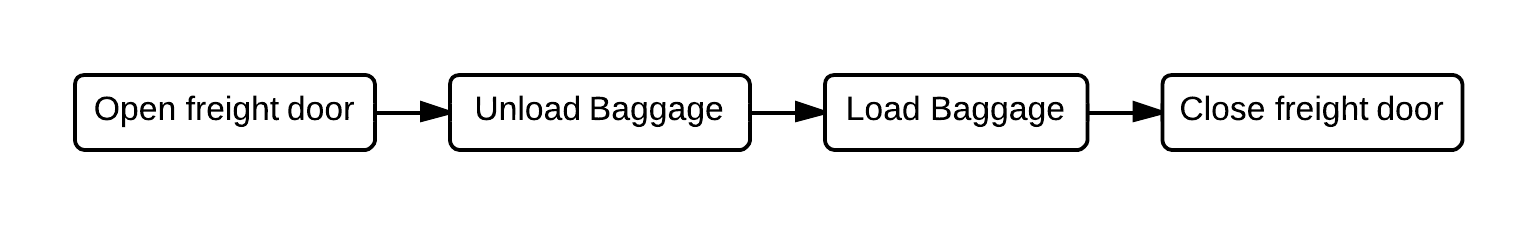
\includegraphics[width=\textwidth]{Grafik/TestCase1Illu}
\end{figure}
\begin{figure}
    \centering
    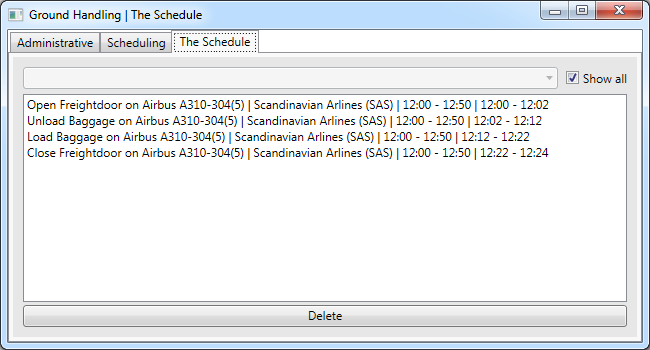
\includegraphics[width=\textwidth]{Grafik/TestCase1Result}
\end{figure}
\end{frame}

\begin{frame}{Test Case 2}
\begin{figure}
    \centering
    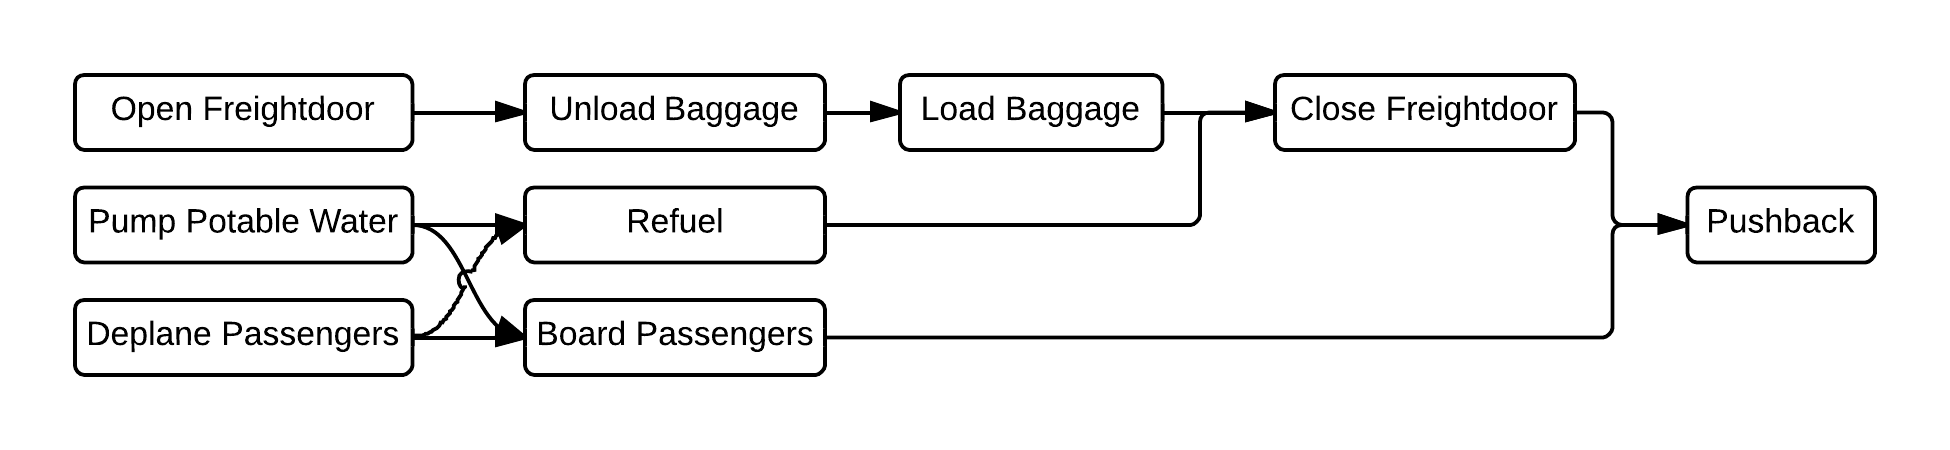
\includegraphics[width=\textwidth]{Grafik/TestCase2Illu}
\end{figure}
\begin{figure}
    \centering
    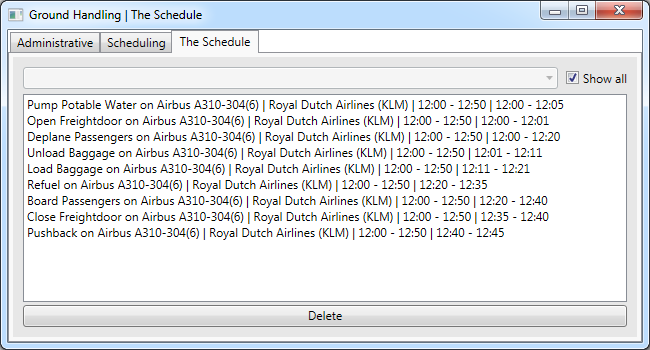
\includegraphics[width=220px]{Grafik/TestCase2Result}
\end{figure}
\end{frame}

\begin{frame}{Test Case 3}
\begin{figure}
    \centering
    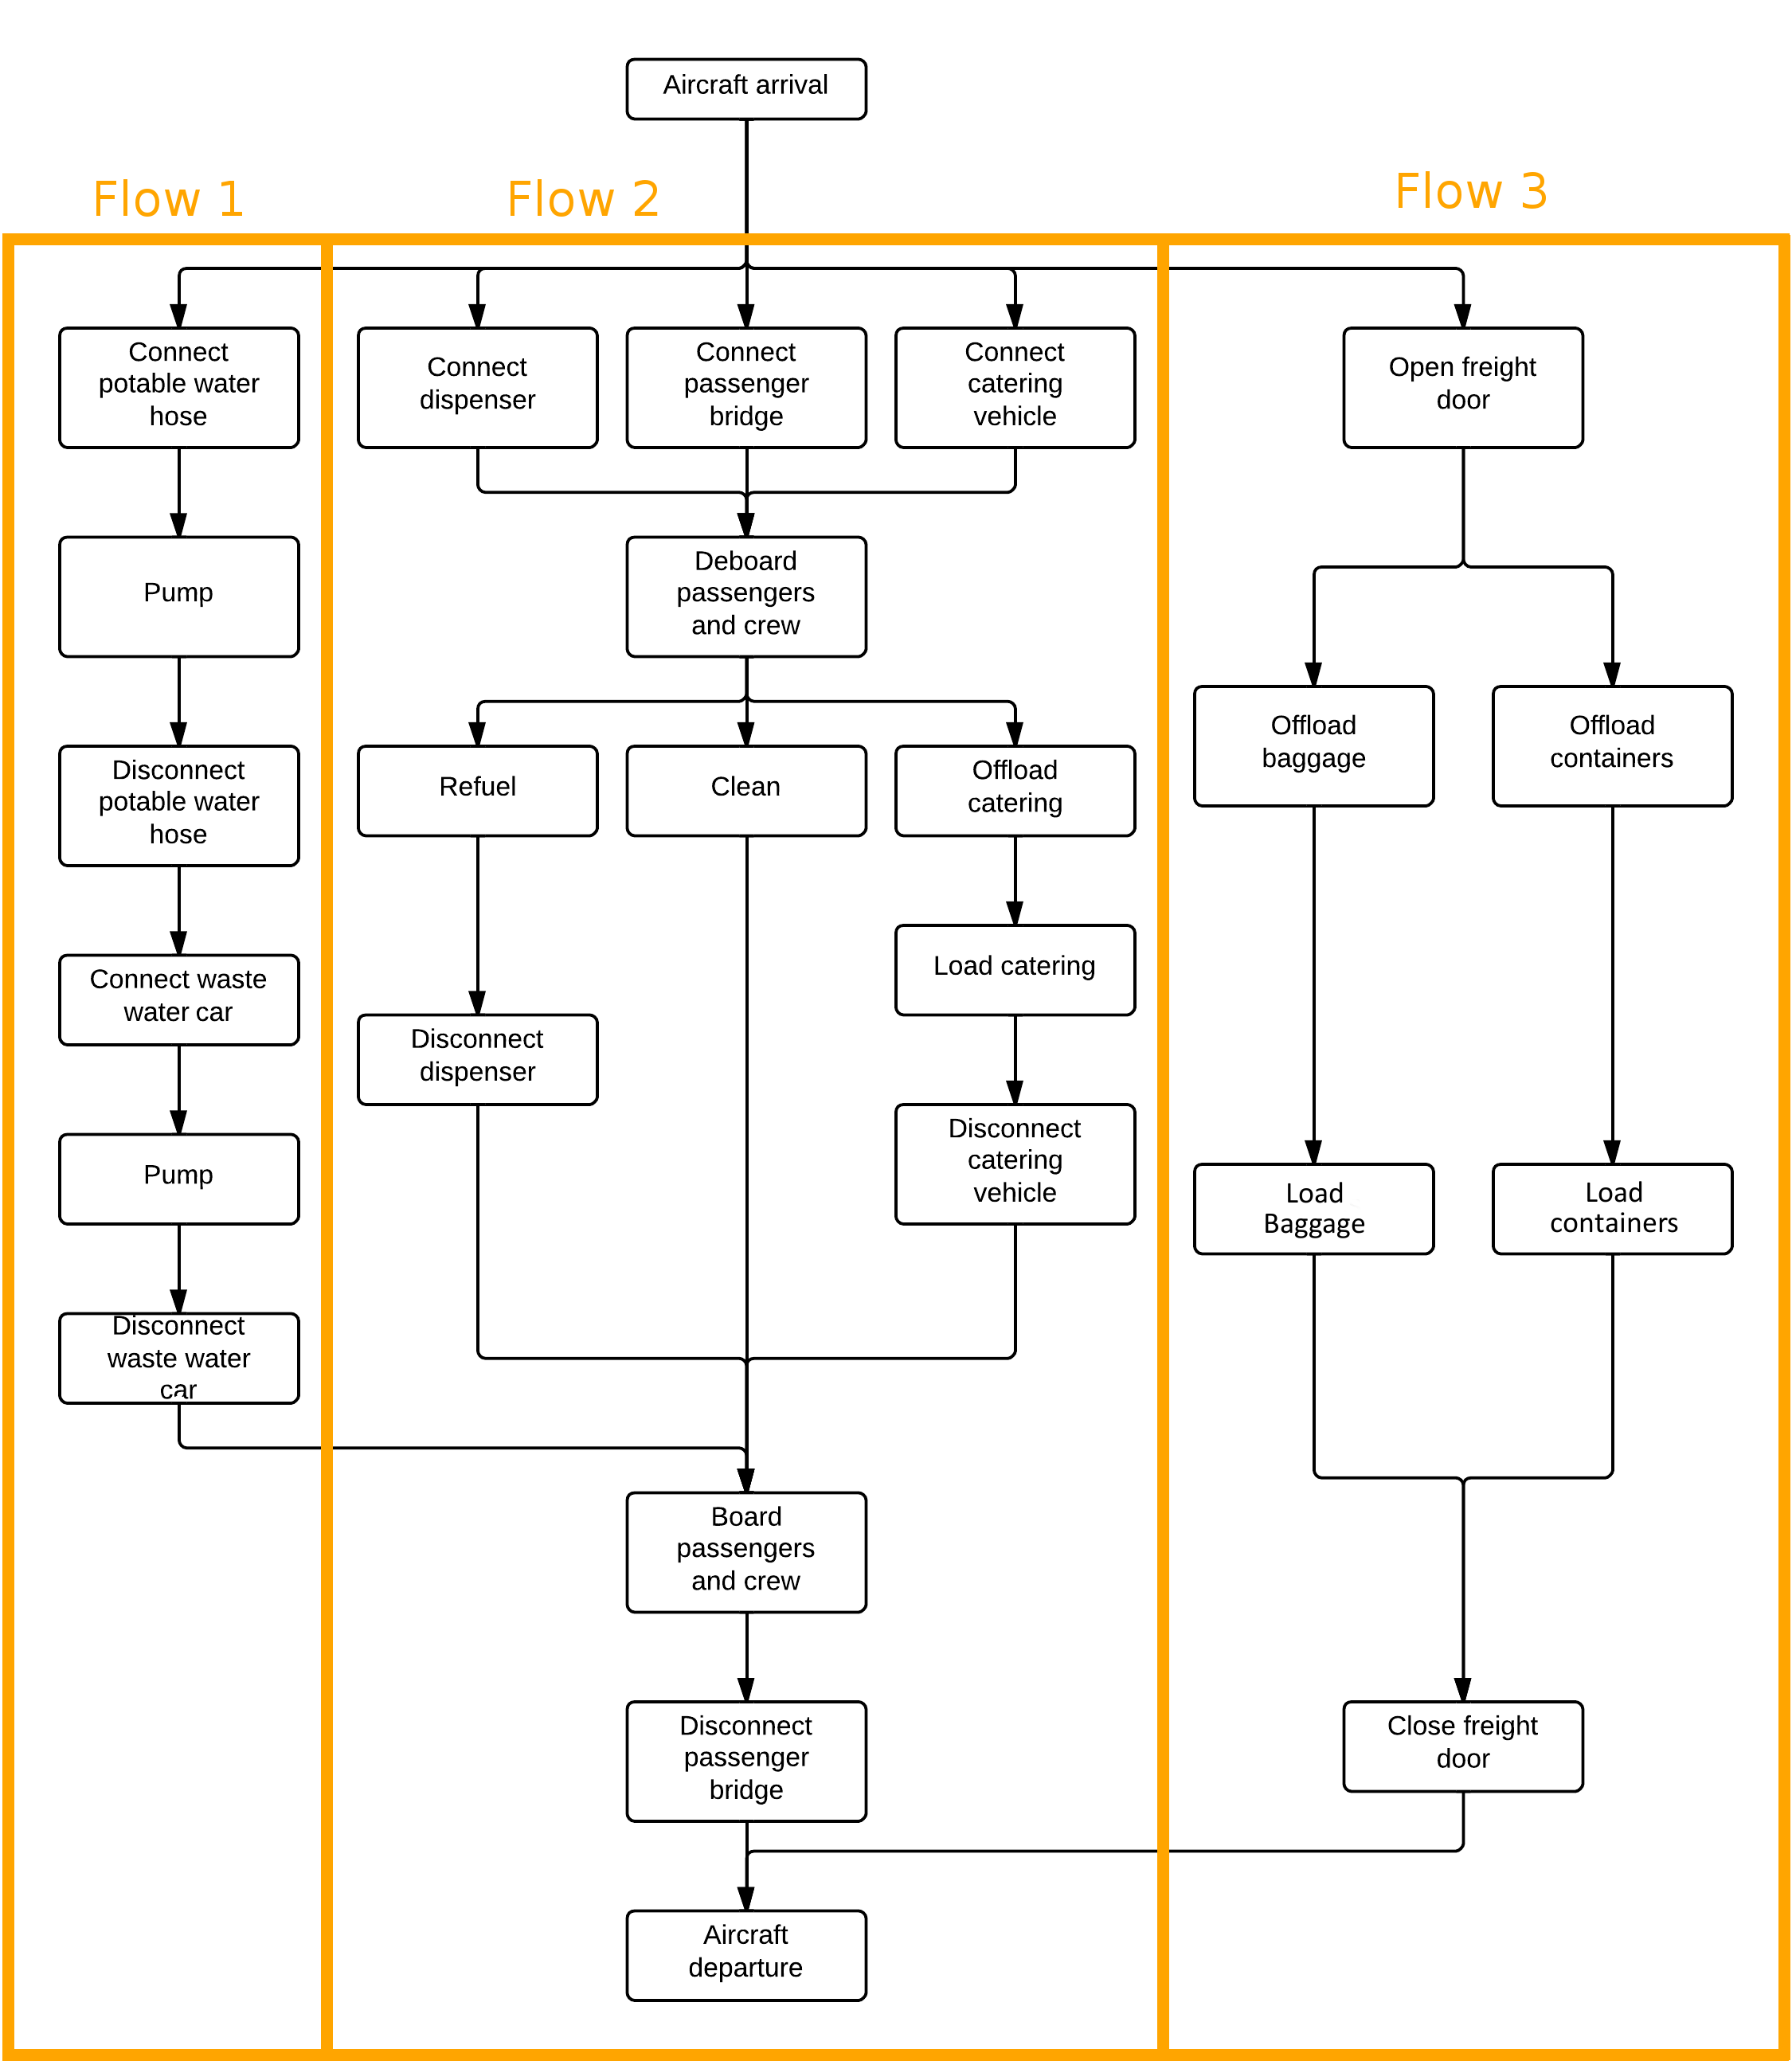
\includegraphics[width=170px]{Grafik/TestCase3Illu}
\end{figure}
\end{frame}

\begin{frame}{Test Case 3}
\begin{figure}
    \centering
    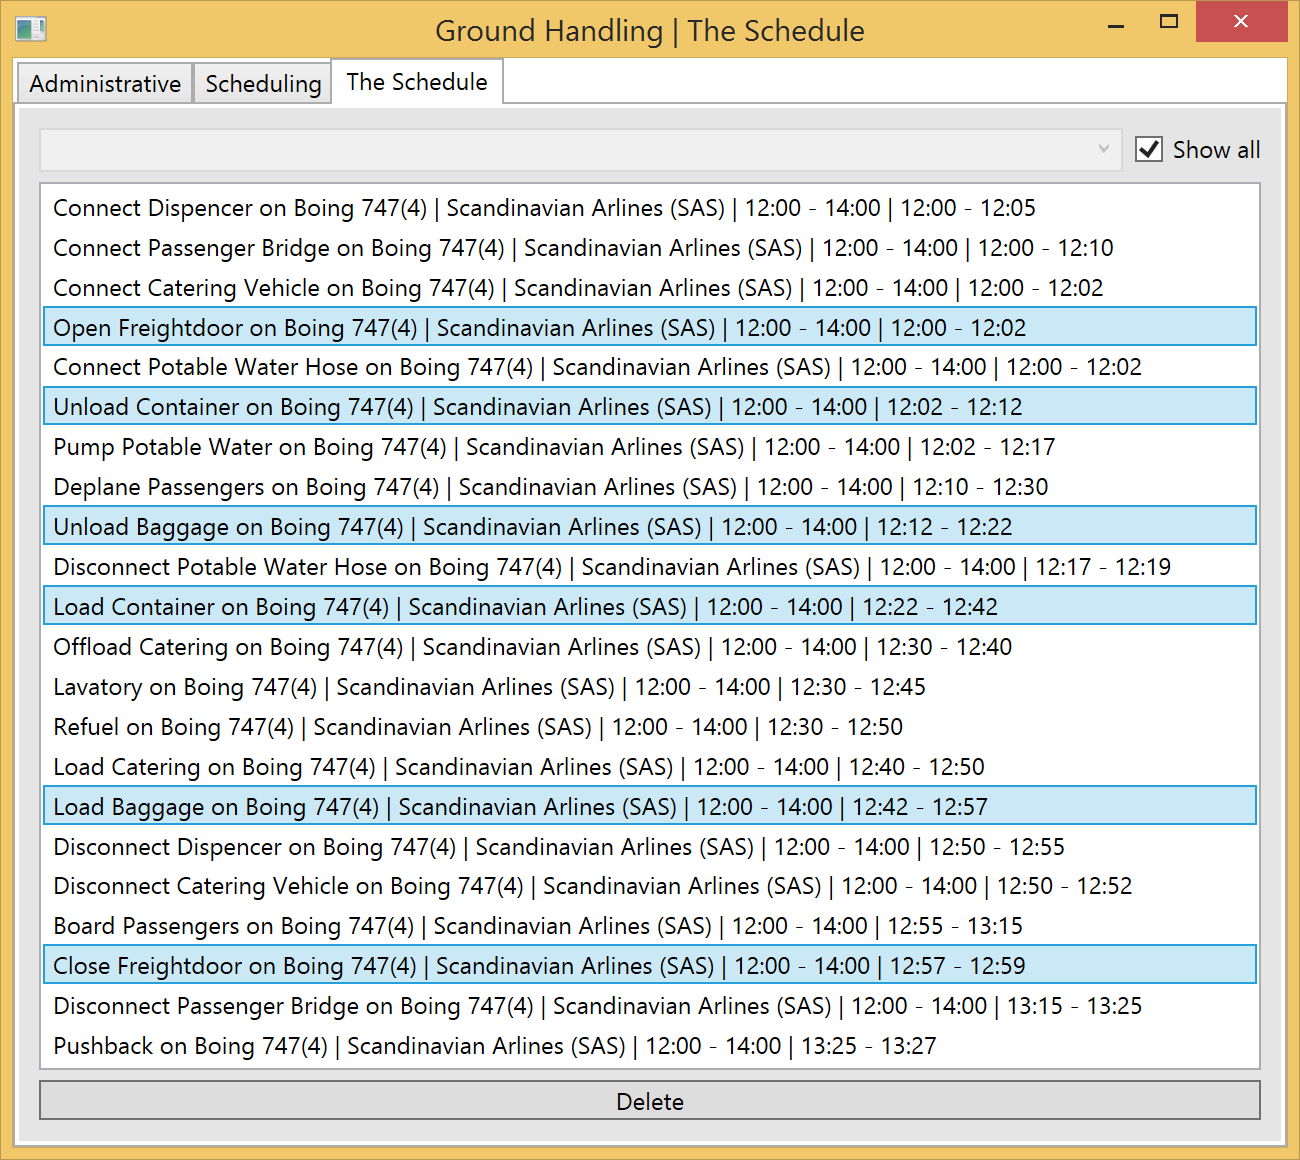
\includegraphics[width=220px]{Grafik/TestCase3Result}
\end{figure}
\end{frame}

\begin{frame}{Test Case 3}
\begin{figure}
    \centering
    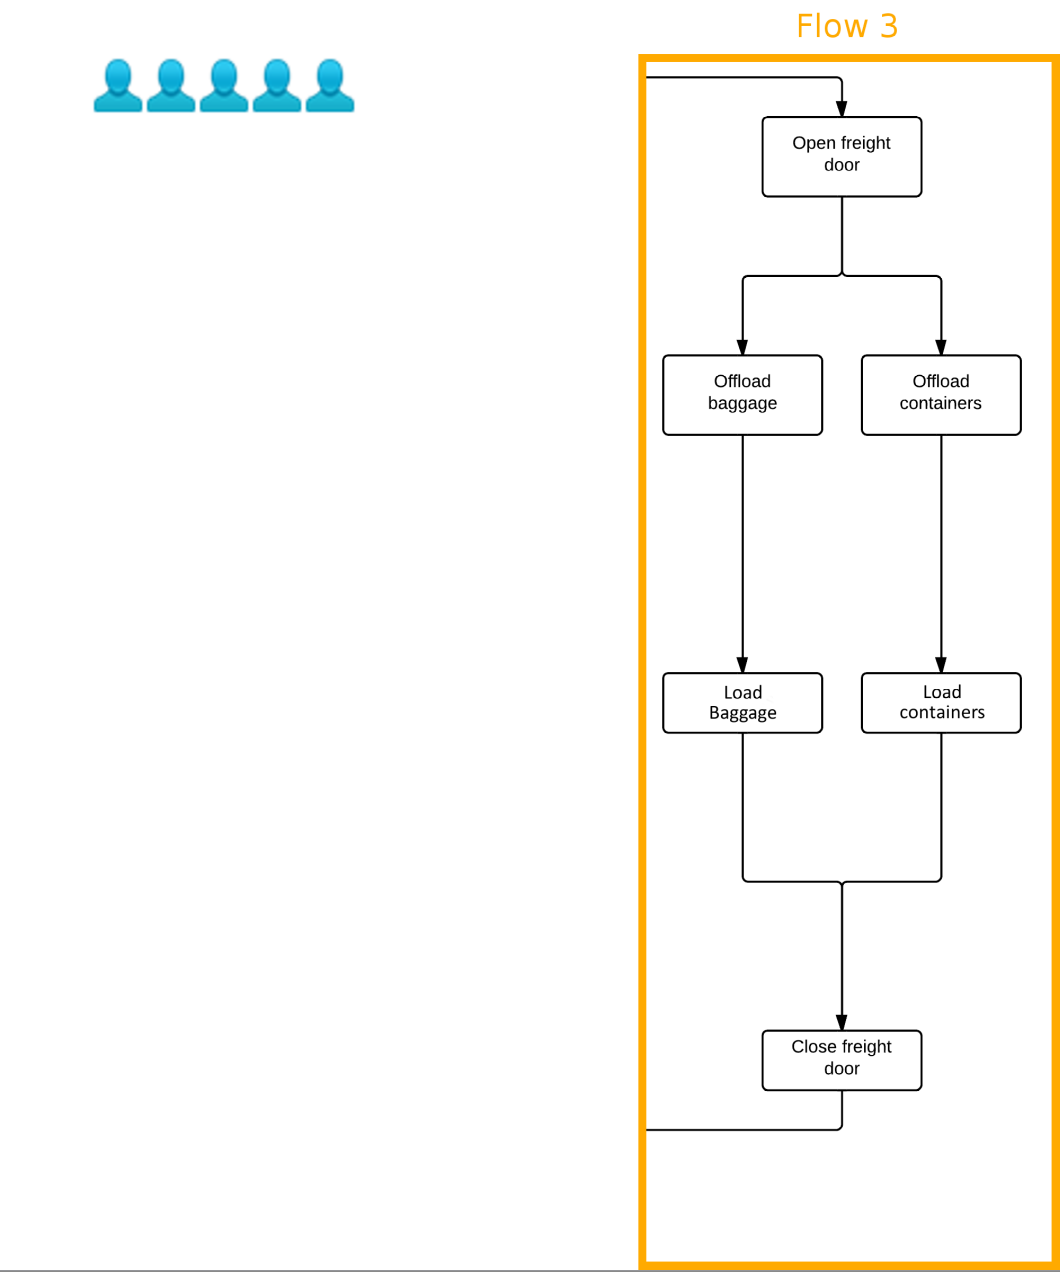
\includegraphics[width=180px]{Grafik/Flow3/Flow3-0-1}
\end{figure}
\end{frame}

\begin{frame}{Test Case 3}
\begin{figure}
    \centering
    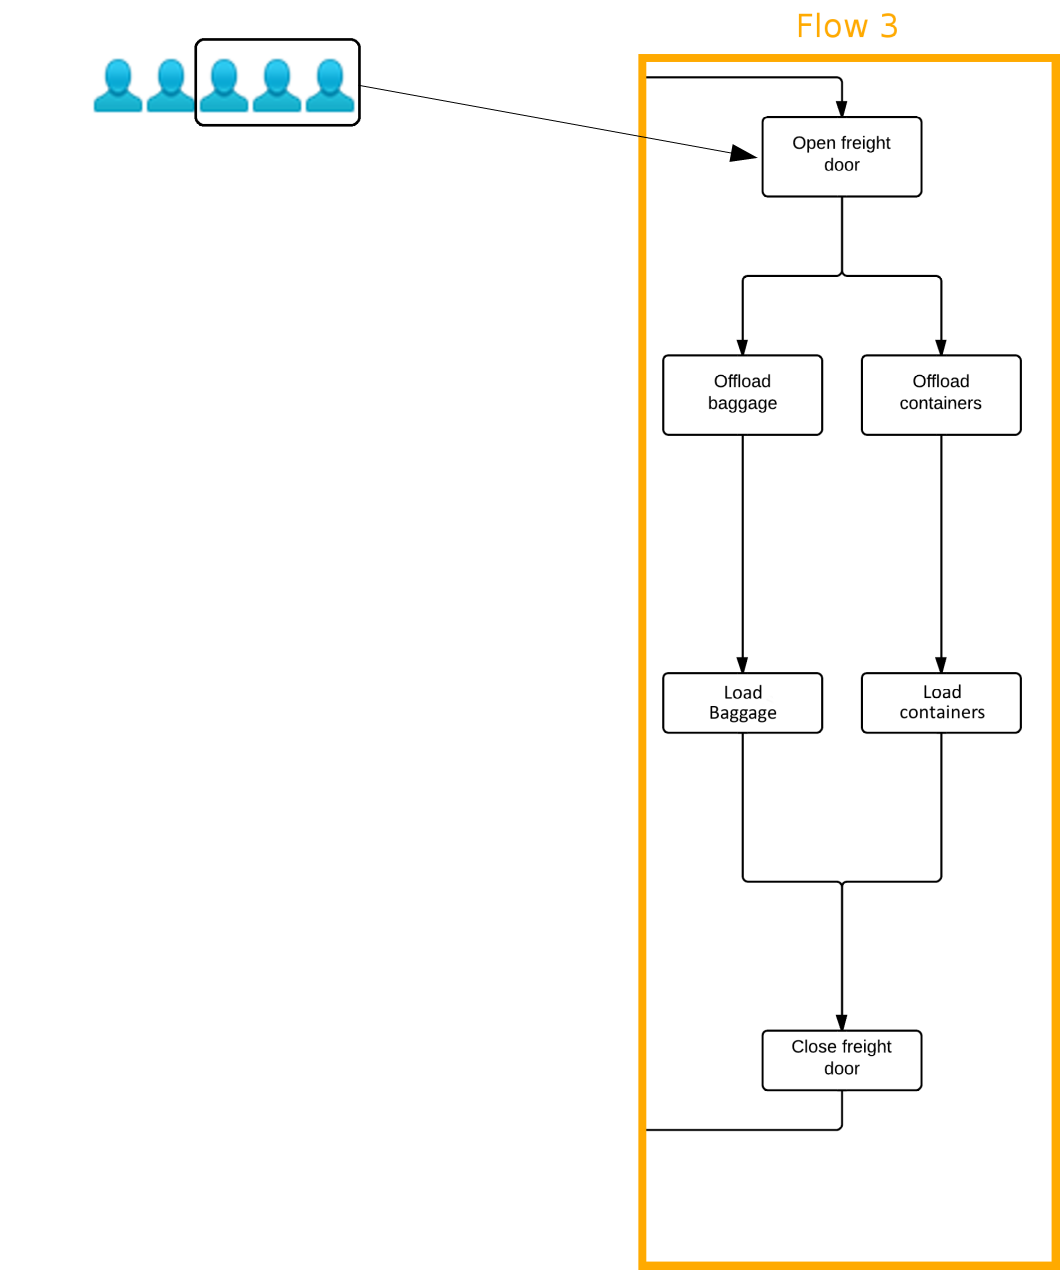
\includegraphics[width=180px]{Grafik/Flow3/Flow3-0}
\end{figure}
\end{frame}

\begin{frame}{Test Case 3}
\begin{figure}
    \centering
    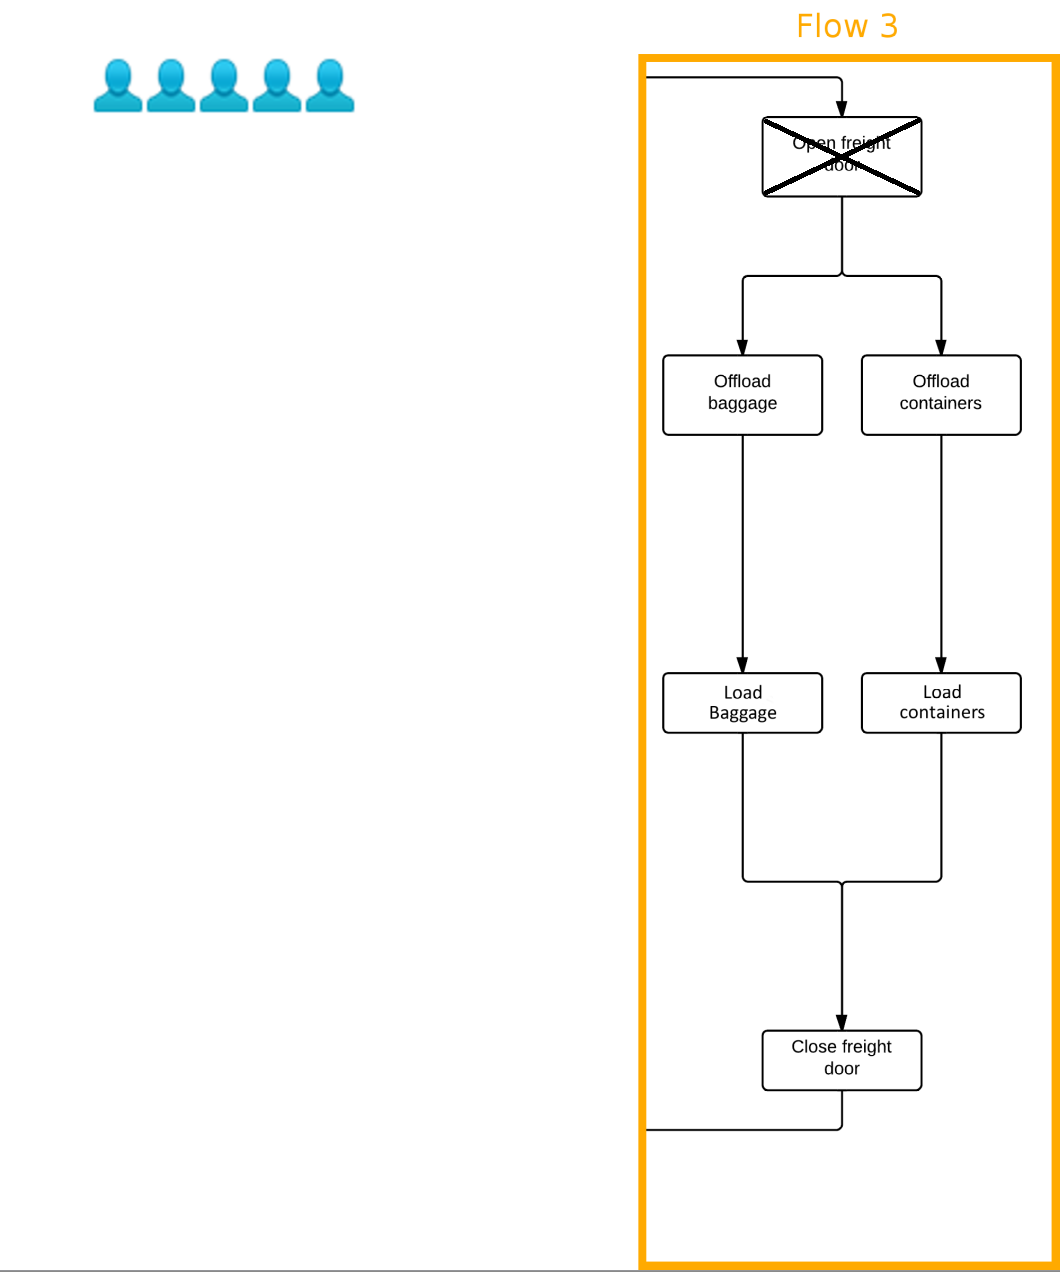
\includegraphics[width=180px]{Grafik/Flow3/Flow3-1-1}
\end{figure}
\end{frame}

\begin{frame}{Test Case 3}
\begin{figure}
    \centering
    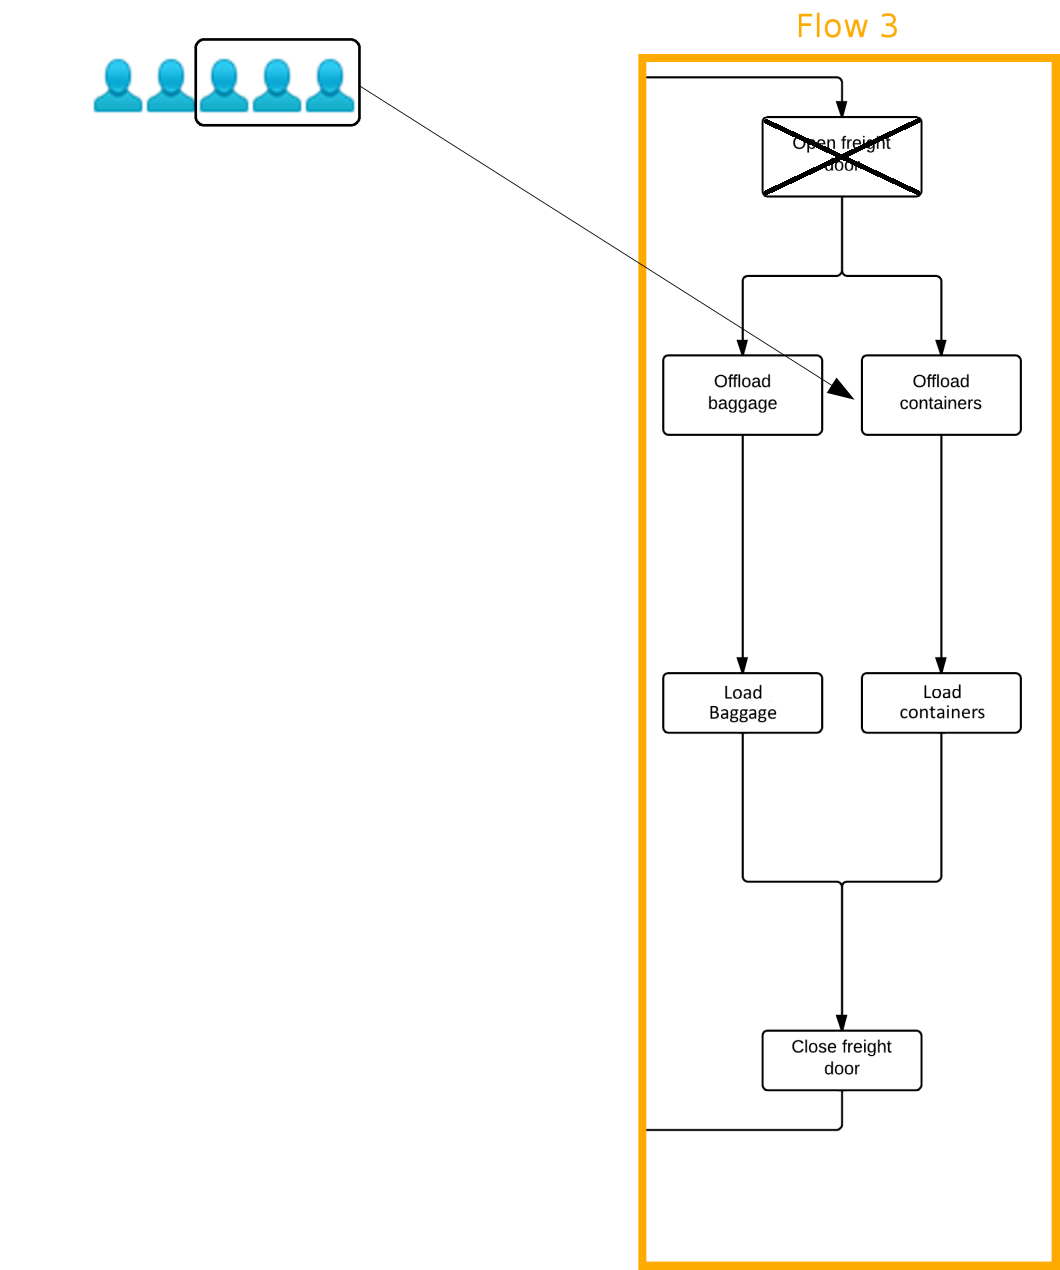
\includegraphics[width=180px]{Grafik/Flow3/Flow3-1}
\end{figure}
\end{frame}

\begin{frame}{Test Case 3}
\begin{figure}
    \centering
    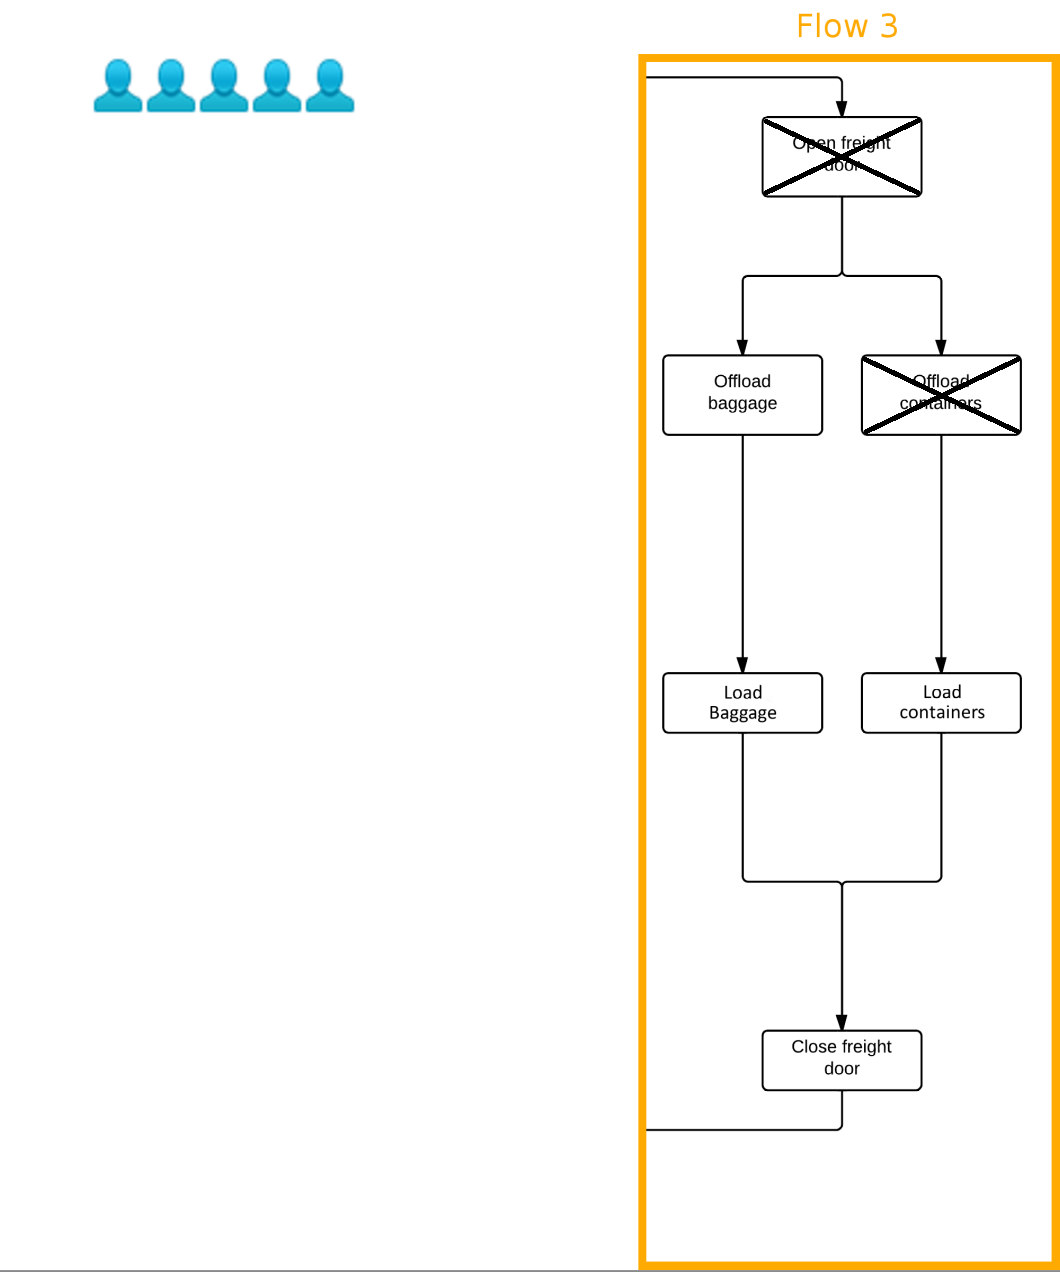
\includegraphics[width=180px]{Grafik/Flow3/Flow3-2-1}
\end{figure}
\end{frame}

\begin{frame}{Test Case 3}
\begin{figure}
    \centering
    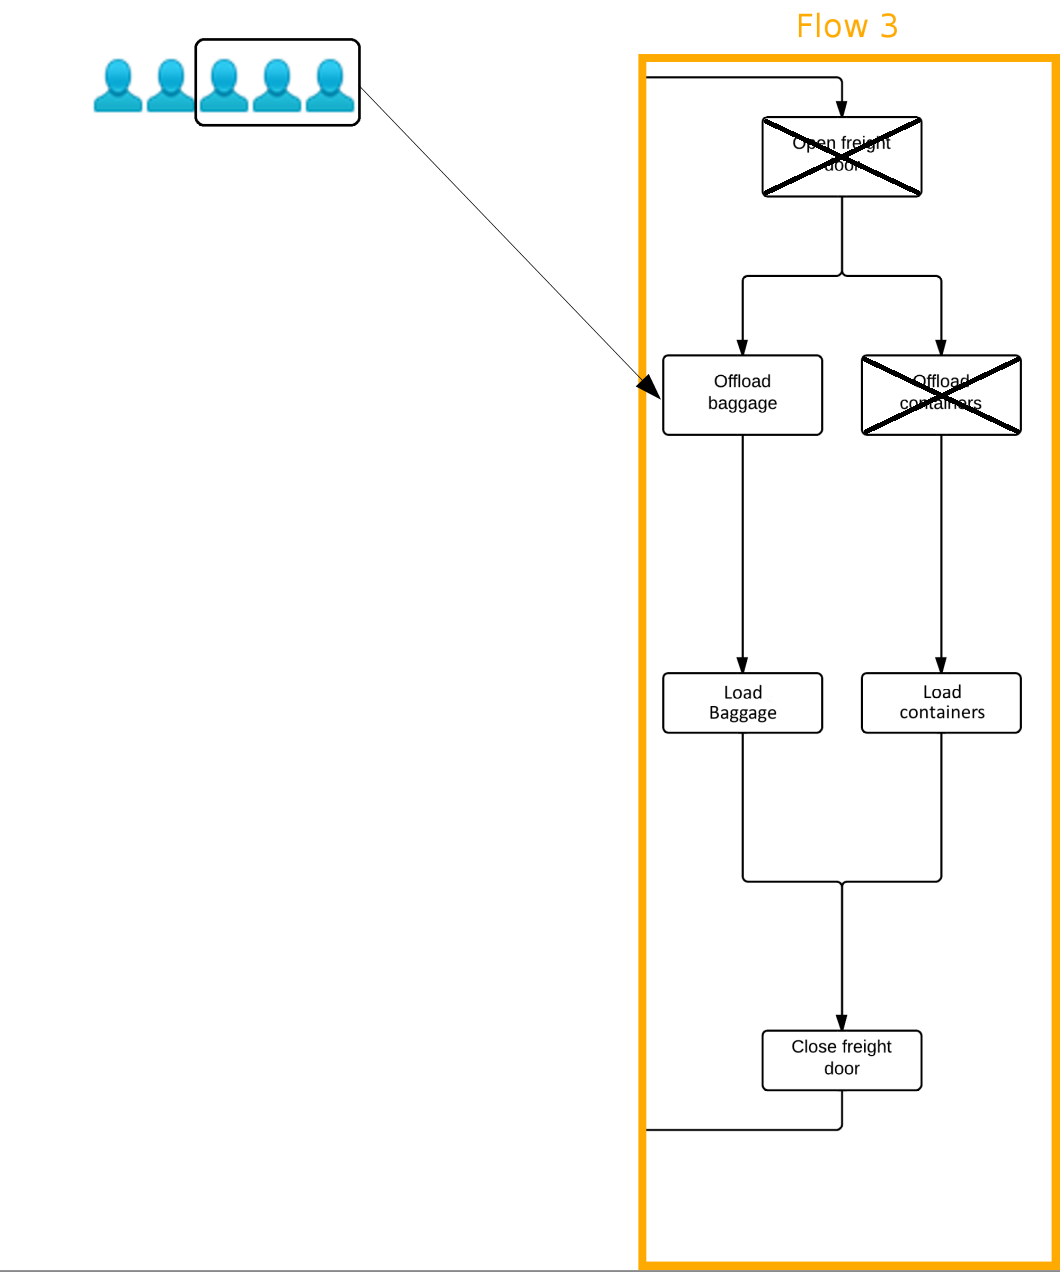
\includegraphics[width=180px]{Grafik/Flow3/Flow3-2}
\end{figure}
\end{frame}

\begin{frame}{Test Case 3}
\begin{figure}
    \centering
    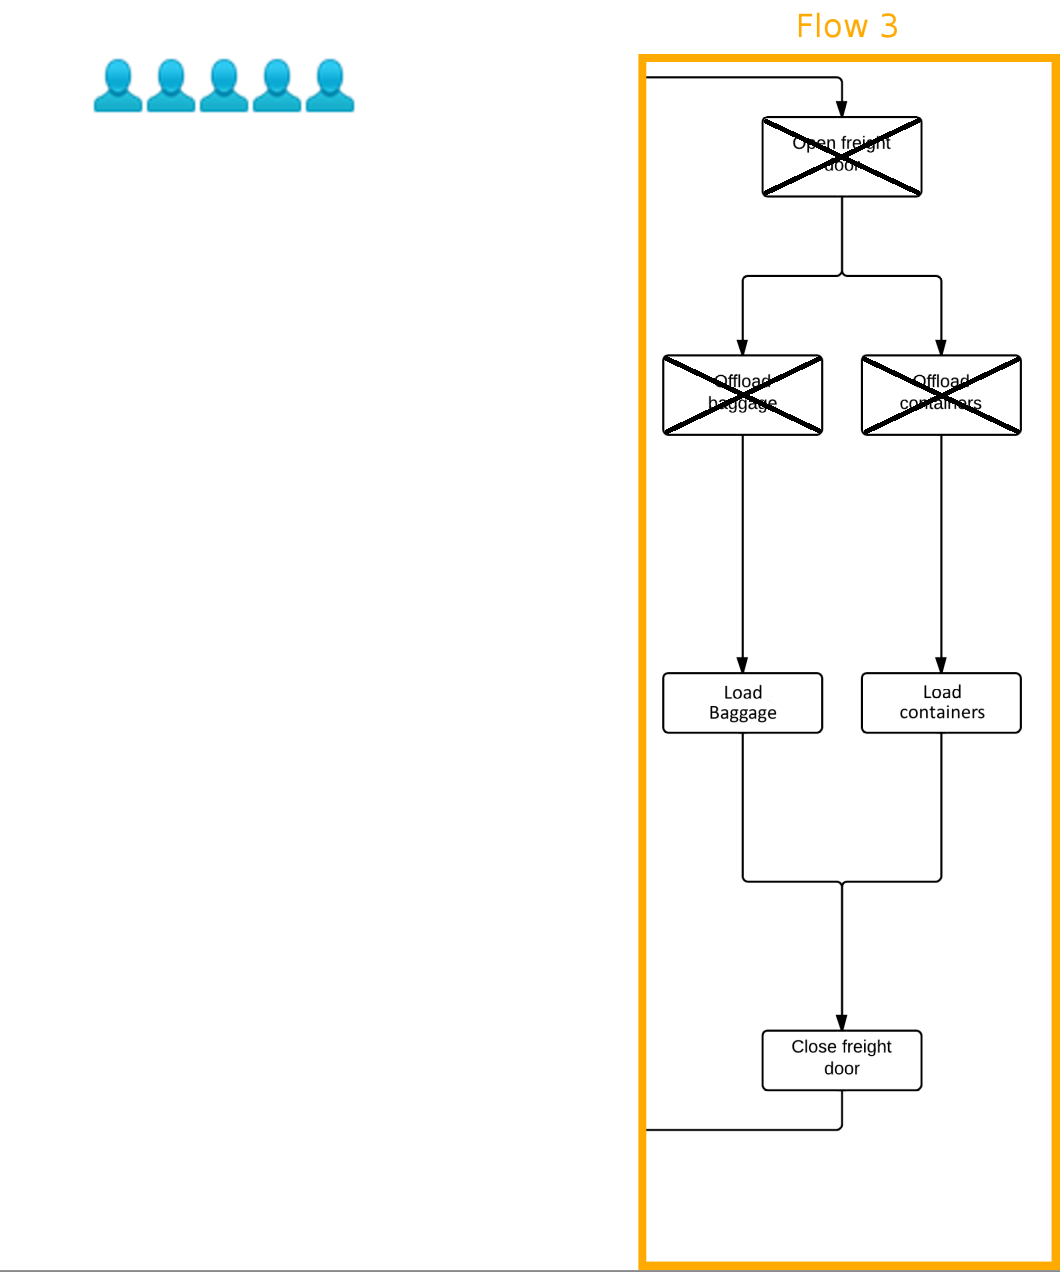
\includegraphics[width=180px]{Grafik/Flow3/Flow3-3-1}
\end{figure}
\end{frame}

\begin{frame}{Test Case 3}
\begin{figure}
    \centering
    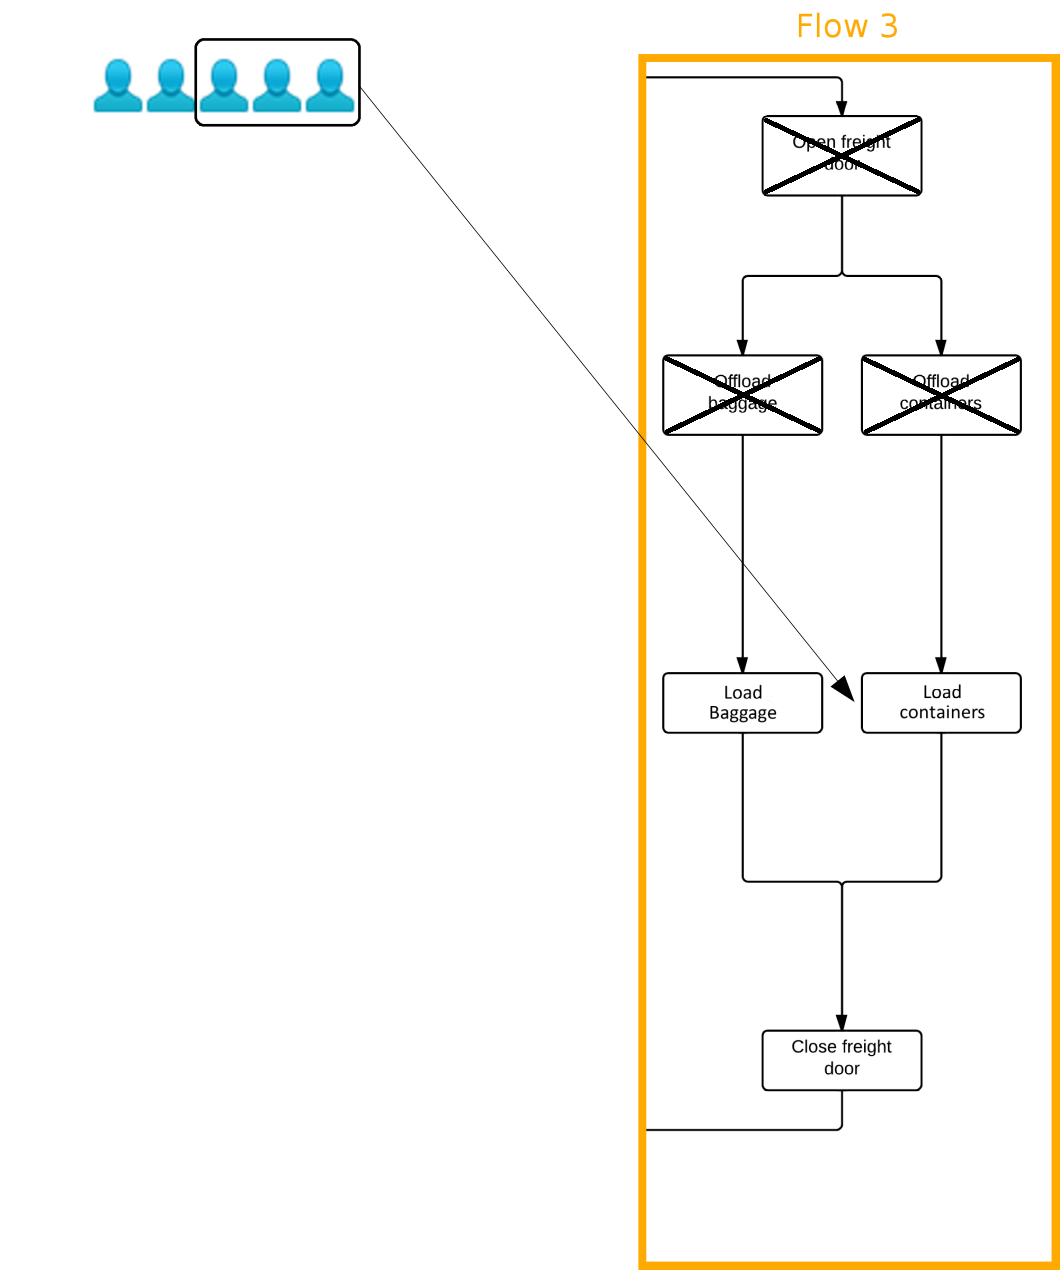
\includegraphics[width=180px]{Grafik/Flow3/Flow3-3}
\end{figure}
\end{frame}

\begin{frame}{Test Case 3}
\begin{figure}
    \centering
    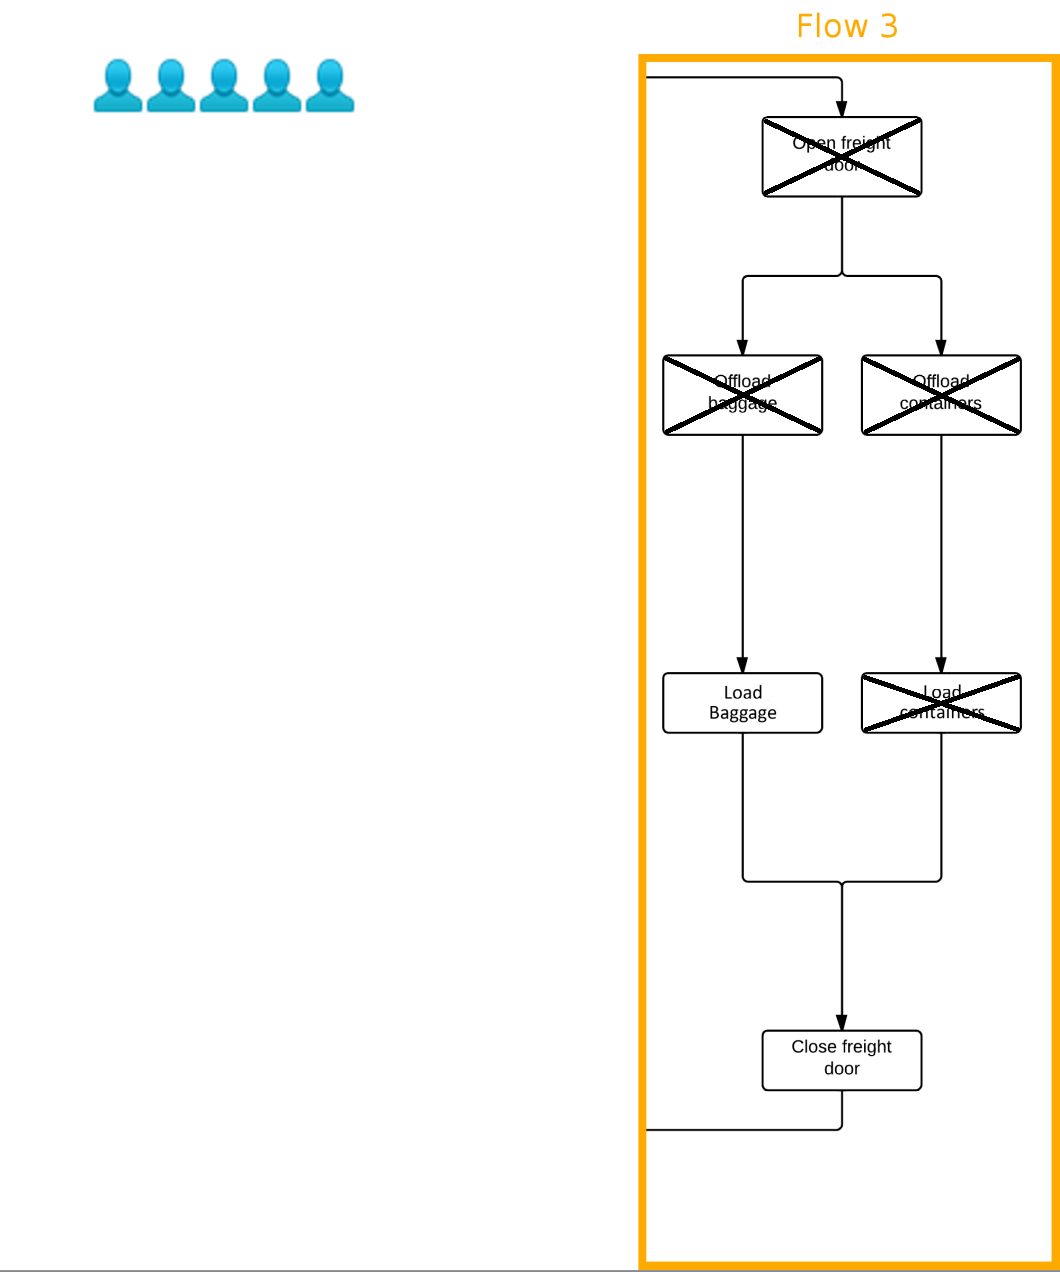
\includegraphics[width=180px]{Grafik/Flow3/Flow3-4-1}
\end{figure}
\end{frame}

\begin{frame}{Test Case 3}
\begin{figure}
    \centering
    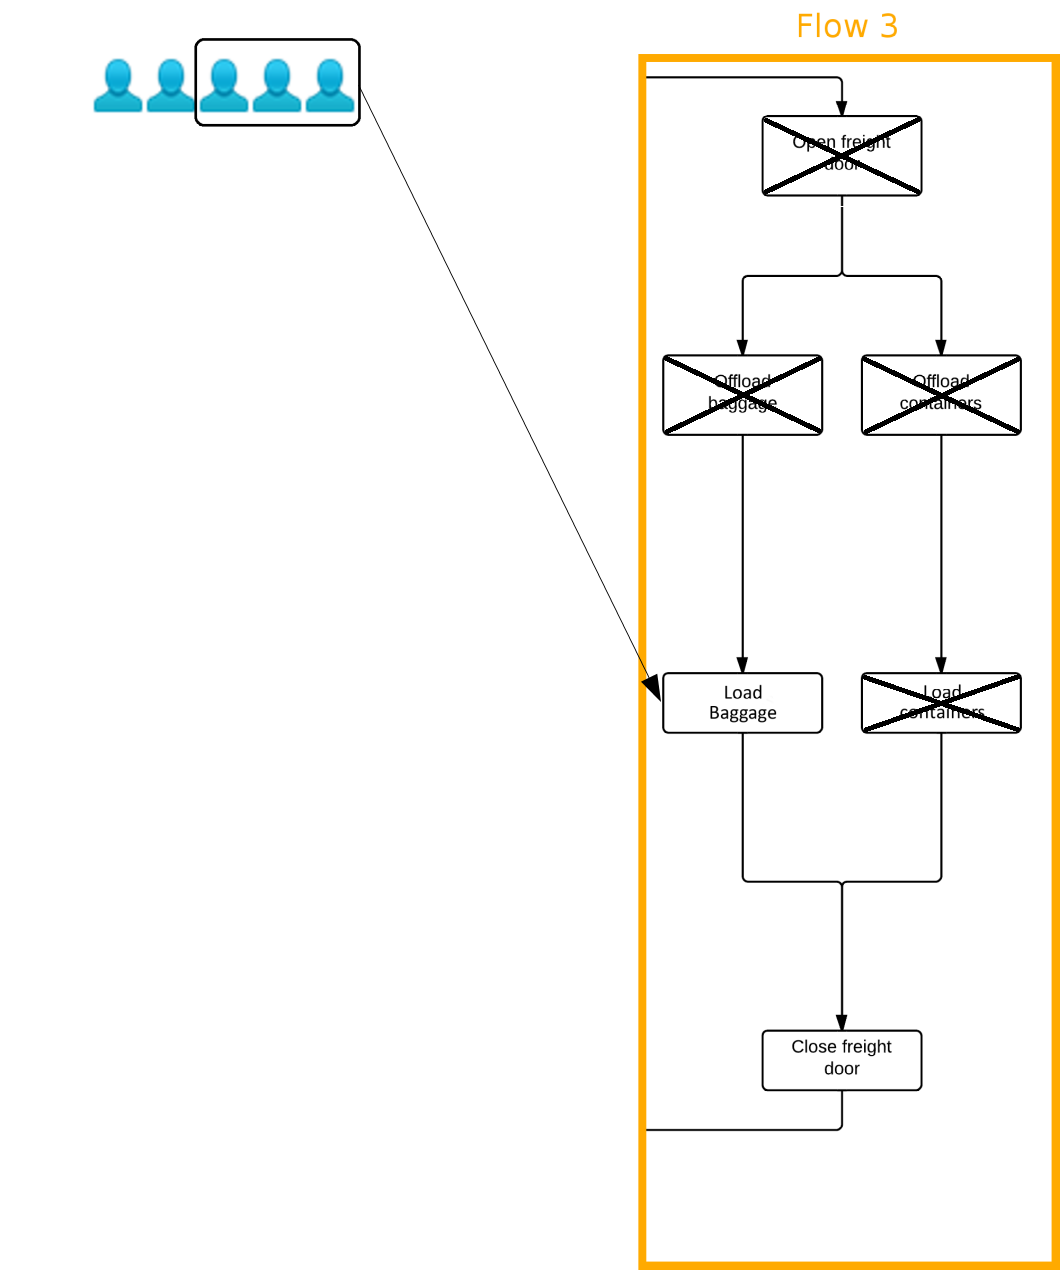
\includegraphics[width=180px]{Grafik/Flow3/Flow3-4}
\end{figure}
\end{frame}

\begin{frame}{Test Case 3}
\begin{figure}
    \centering
    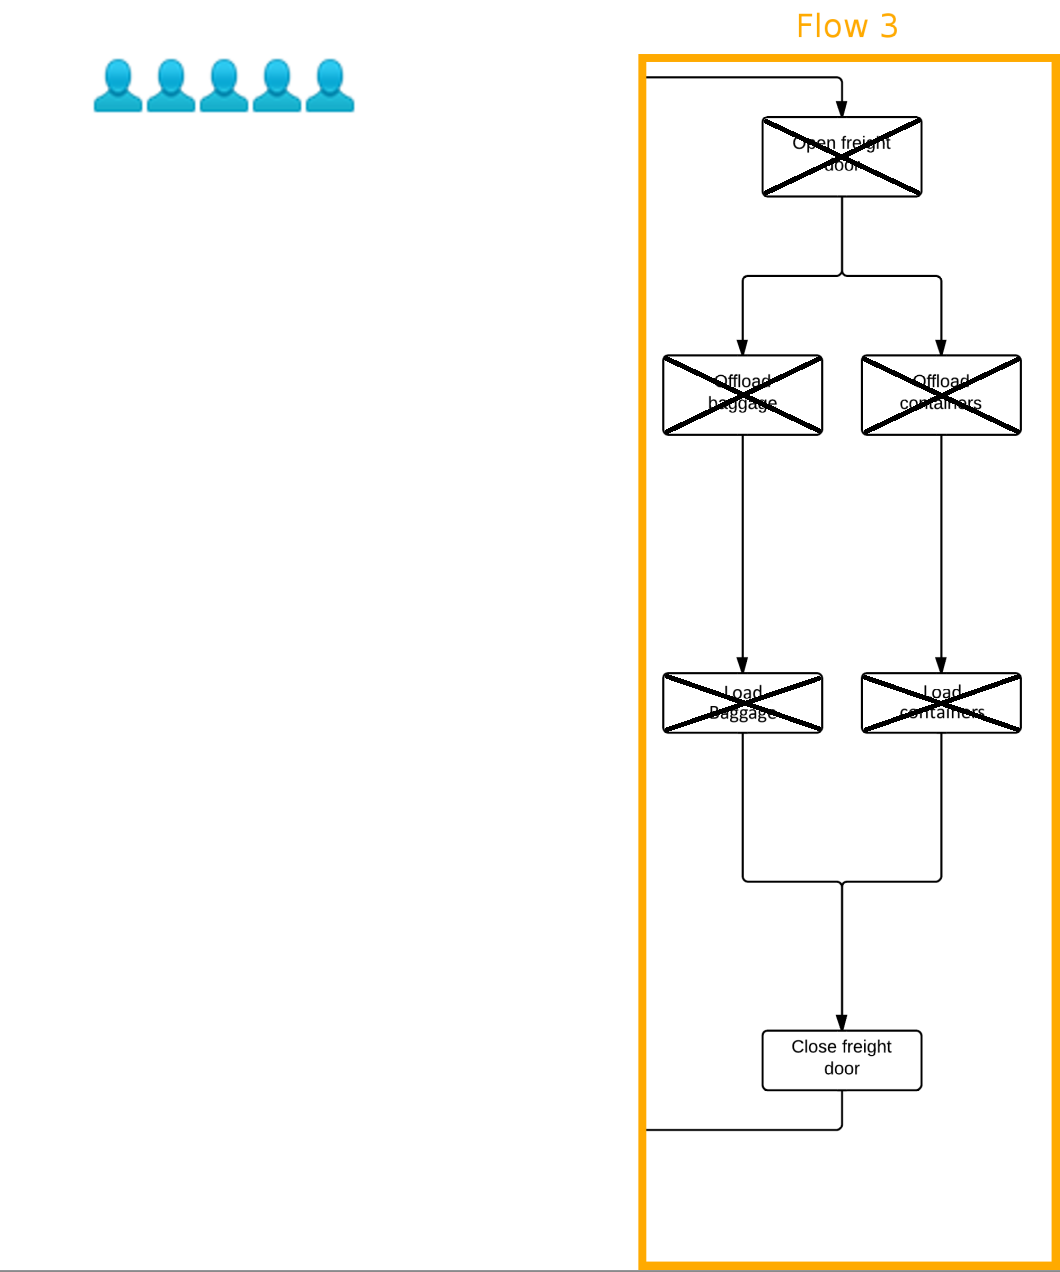
\includegraphics[width=180px]{Grafik/Flow3/Flow3-5-1}
\end{figure}
\end{frame}

\begin{frame}{Test Case 3}
\begin{figure}
    \centering
    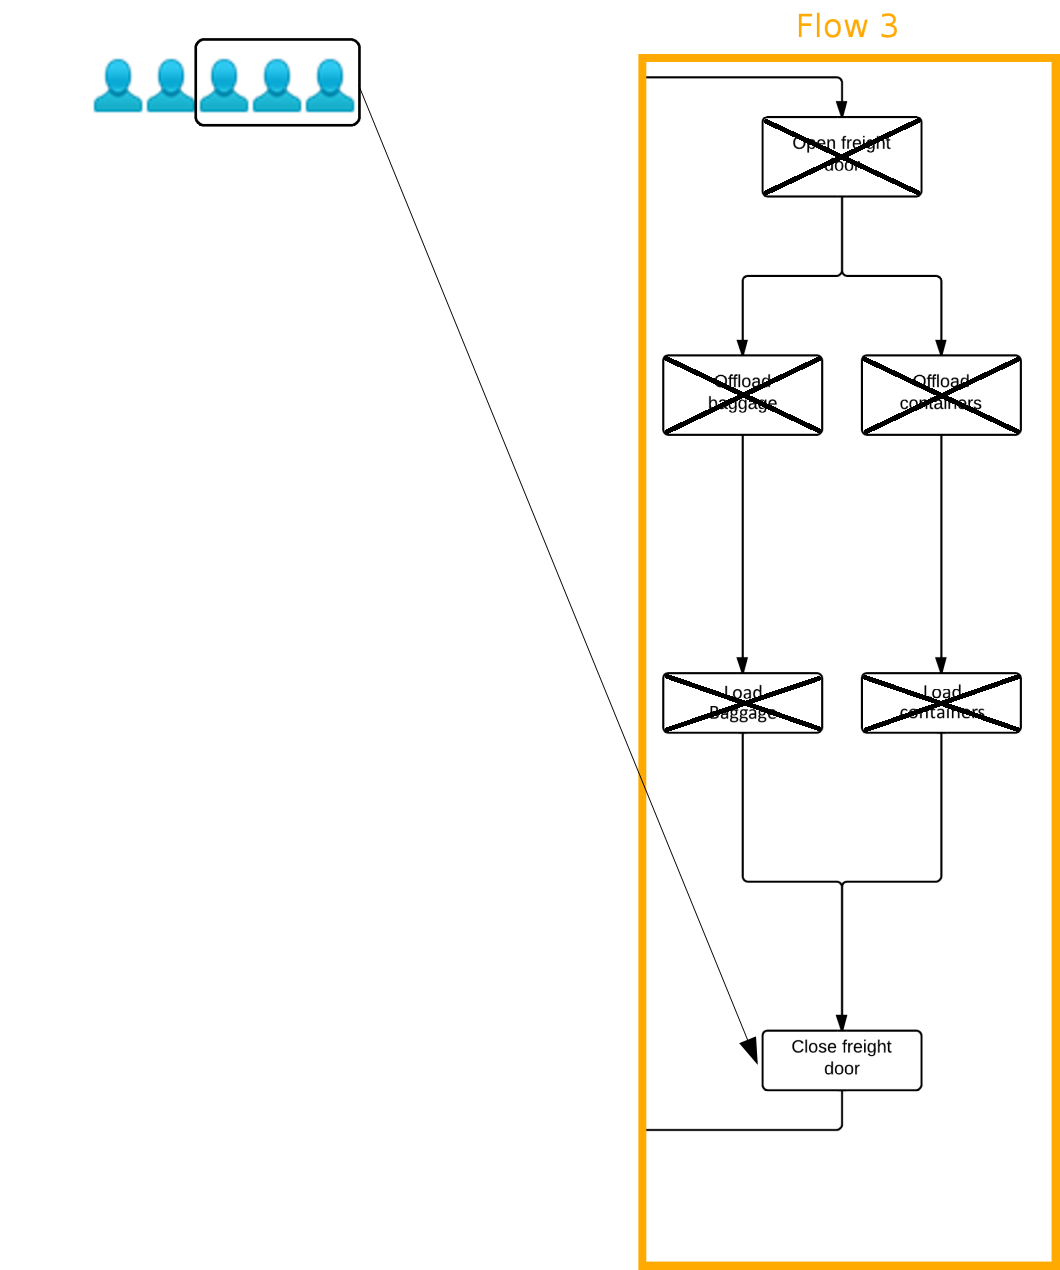
\includegraphics[width=180px]{Grafik/Flow3/Flow3-5}
\end{figure}
\end{frame}

\subsection{Complex Test Case}
\begin{frame}{Complex Test Case}
\begin{itemize}
\item 30 flights
\item All planes delayed a bit vs few planes delayed a lot
\begin{itemize}
\item A small plane will always be set aside for a large plane if there are not enough workers
\end{itemize}
\end{itemize}
\end{frame}

\subsection{Complexity}
\begin{frame}{Complexity}
\begin{itemize}
\item Most Critical Path
\begin{itemize}
\item $O(n*log(n))$
\item $O(n^2)$
\end{itemize}
\item Brute Force Search
\begin{itemize}
\item $O(n!)$
\end{itemize}
\end{itemize}
\end{frame}

\subsection{Scaling}
\begin{frame}{Scale Test Case}
\centering
$f(x) = 0.59x^2 - 17.8x + 141.6$
\begin{figure}
    \centering
    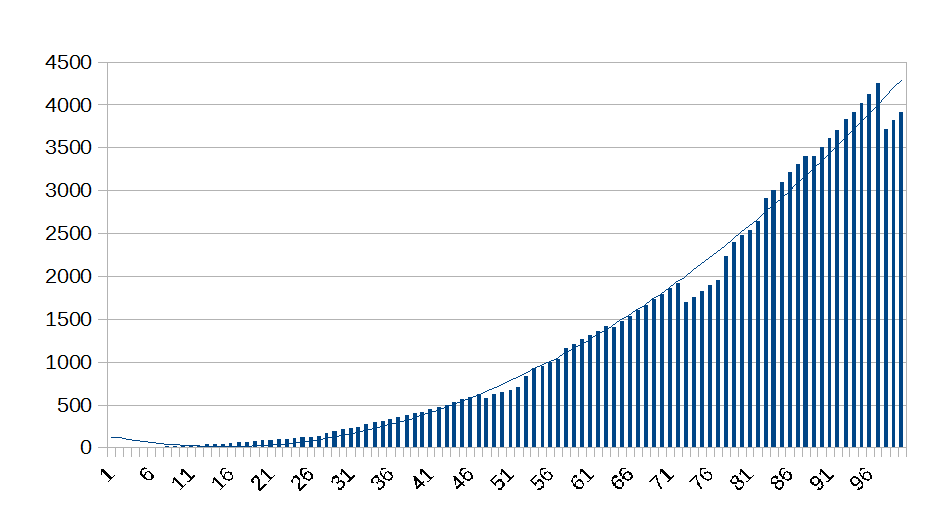
\includegraphics[width=\textwidth]{Grafik/ScaleTestResult}
\end{figure}
\end{frame}

\subsection{Summary}
\begin{frame}{Summary}
\begin{enumerate}
\item If the choice stands between two identical workers, the one who has done the least amount of work should be taken
\item If the choice stands between two or more equally critical flows, where only one can be worked at at the time, the one flow should be completed before the other(s) is/are started (no alternating)
\item More or fewer workers than one exact amount, should be able to be assigned to a task and the task 
\item The last tasks on an airplane and tasks on a small airplane are prioritized low, resulting in that flights may be delayed, this could be solved by
\begin{enumerate}[a)]
\item Modeling the graph where all airplanes are in one large graph, where departure time of the airplane adds to the weight
\item A dynamic prioritization list where the weight is work-minutes required to complete the flight over time remaining
\end{enumerate}
\end{enumerate}
\end{frame}